\documentclass[twoside,12pt,titlepage,a4paper]{article}
\usepackage{url}
% kentHarvard requires natbib
\usepackage{natbib}
% add line numbers
% TODO: remove line numbers and run minted for release
\usepackage{lineno}
% \usepackage{minted}
\usepackage{etoolbox}
\makeatletter
\patchcmd{\@verbatim}
{\verbatim@font}
{\verbatim@font\scriptsize}
{}{}
\makeatother
\usepackage[final]{pdfpages}
\usepackage{xcolor}
\linenumbers
\definecolor{periwinkle}{rgb}{0.8, 0.8, 1.0}
\renewcommand{\linenumberfont}{\normalfont\bfseries\small\color{periwinkle}}
\usepackage[pass]{geometry}
\usepackage{graphicx}
\renewcommand{\baselinestretch}{1.3}
\usepackage{todonotes}
\usepackage{hyperref}
\usepackage[autostyle]{csquotes}
\setcitestyle{numbers}
\setcitestyle{square}

\title{Usage and Structure of continuous integration as configuration?}
\author{Joseph Ling\\\vspace{10mm}
\url{jl653@kent.ac.uk} \\ \vspace{5mm}

\includegraphics[scale=0.6]{Kent_Comp_294_RGB} \\
School of Computing \\
University of Kent \\
United Kingdom \\ \vspace{10mm} \\ Word Count: around 5500}
\begin{document}

\newgeometry{hmarginratio=1:1}    %% make layout symmetric
\maketitle
\restoregeometry              %% restore the layout

\begin{abstract}
  Continuos integration (CI) is becoming more popular as software development moves to an Agile fast paced development life cycle. Most CI is done automatically using a service which run based off configuration. Our major questions is how much is CI actually being used? As well as how are these files being structured? We got 31,494 open source projects from Github to answer these questions. In doing so compared our results against \citet{Hilton2016} work to see if their has been a increase in usage. We found a shift in CI services being used and were able to get similar results to their study. In terms of structure we found that configuration files are written with no comments normally. We suggest at the end further research is needed to get a better understanding of this growing field.    
  \todo[]{similar is a bad word to use to describe the comparison}
\end{abstract}

\section{Introduction}
\label{Introduction}

Continuos integration (CI) is becoming more popular over the last few years. This can be seen by how major version control hosting services Github, Bitbucket and Gitlab have all started to or have been improving their CI products. In terms of research, Infrastructure as Code in \citet{Rahman2019} which does a systematic mapping of research in that area. For Continuous Integration with \citet{Shahin2017} which does another systematic review on how it is used. These two papers demonstrate some of breadth of research that has taken place. In addition you have papers like Google's Innovation Factory: Testing, Culture, and Infrastructure \citet{Copeland2010} which demonstrate some of the depth that the papers go into.
\todo[]{google paper might not be the best one here, we want to demonstrate reading around the area here but not too include a paper which we will go into much later but is still relevant}

Continuos Integration is a process of automatically running compiling, running tests and checking that the product works. This is can be combined with Continuos Delivery where the product is deployed or released after it has gone through successfully CI. 

This can get complicated quickly therefore Configuration as Code (or Infrastructure as Code) is used to configure it. The main kind of configuration format used for this is Yaml followed by Xml and Java based scripting formats.


In order to look at our first theme CI usage we looked at In Usage, Costs, and Benefits of Continuous Integration Open-Source Projects \cite{Hilton2016}. They looked closely at usage of CI as well. As we are looking at CI usage as well we are going answer the first three questions from their theme \enquote{Usage of CI}. 
\begin{itemize}
  \item \textbf{RQ1} What percentage of open-source projects use CI?
  \item \textbf{RQ2} What is the breakdown of different CI services?
  \item \textbf{RQ3} Do certain types of projects use CI more than others?
\end{itemize}

However the two key differences is that we will be scraping a new data set for the comparison. In doing so gathering slightly more data on the repositories but not none on pull requests. As well as we didn't conduct a survey. From that additional data we are going to look more closely at the first question of What percentage of open-source projects use CI?
As we are asking the same questions, we will use their corpus to compare on what has changed over the last 4 years. 
For our second theme, structure of CI as configuration we wanted to pick structural components that would be similar between all CI files. It would have been really interesting to do a full in depth analysis of each like \citet{Gallaba2018}. However we would like to tie in how the files are structured to how they are used so won't following that style. This led to the following research questions:
\begin{itemize}
  \item \textbf{RQ4} What are the common errors when loading yaml configuration?
  \item \textbf{RQ5} How are comments used in the configuration?
  \item \textbf{RQ6} How are external scripts used within the configuration?
\end{itemize}

\section{Related Works}
\vspace*{-0.05in}
\subsection{Continuos Integration}
\vspace*{-0.05in}

Continuos Integration is frequently submitting work normally tied into a feedback loop. For example using version control and committing changes daily. For each changed committed a server builds and tests the changes informing you of status of those changes. As well as providing a build which is typically a binary executable of code that can then be saved if necessary. In doing you can reduce the chances of facing the situation off "It works on my machine...". As the building and packaging of the code is done on a server to make sure everything integrates.

An early definition of CI was written up and then updated later by Martin Fowler \cite{CI2010_MartinFowler}. A key part of the CI is that allows teams to work on the same code base which without CI could easily lead to integration bugs and broken builds. 

To enable to this to happen automation needs to put in place for build, testing and other aspects of the integration process in order that a clear piece of feedback (yes or no) can be given about the status of the build. If done with from a version control system if the same commit is built twice (so no changes have happened) it is vital that it produces the same result. Otherwise it is hard for a team to be able to depend on CI if they are getting flakey test results or flakey build results.

\vspace*{-0.05in}
\subsection{Usage of Continuous Integration}
\vspace*{-0.05in}

The actual usage of CI as configuration was looked at by \cite{Hilton2016}. In this they use three source of information Github repositories, Travis builds and a survey. In order to be do a more systematic study of CI usage than \cite{Vasilescu2015}. In analysing that data they found that "The trends that we discovered point to an expected growth of CI. In the future, CI will have an even greater influence than it has today." As we are looking at the same question we will use four of the research questions out of the fourteen. In order to see what difference four years has made to the growth of usage of CI.

\vspace*{-0.05in}
\subsection{Config as code}
\vspace*{-0.05in}

Configuration as code or Infrastructure as Code has been an increasing area of research over the last few years. There seems to be slightly more research in infrastructure as code \citet{Rahman2019}. The has been a focus on Puppet and Chef, for example in \citet{Sharma2016} looks at code quality by the measure of \enquote{code smell} of Puppet code. This tackles the problem by defining by best practices and analyzing the code against that. In the case of \citet{Cito2017} it uses the docker linter in order to be able to analyse the files. 
For the CI systems we pick we will look into the tooling around that to aid the analysis.


\section{Methodology}
\label{methodology}
% here we want to describe why we went with Github over GhTorrent 
In order to answer the research questions we needed to find projects for CI configuration files. This is because we needed to get the contents of the configuration in order to analyse the structure of it. We chose to scrape Github via their Api as it was easy to setup and test whether or not it was working as there is a 121 mapping between the api and user interface. However using Ghtorrent \citet{GhTorrent2020} it may have been easier to gather more data because the rate limiting wasn't as strict. Yet harder to test whether or not it is working. Therefore we decide to use the Github Api as the source for our corpus.

\begin{figure}[!htbp]
  \centering
  \begin{minipage}{.48\textwidth}
    \centering
    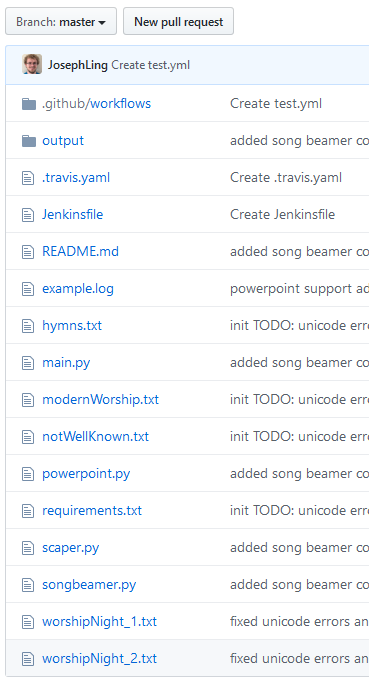
\includegraphics[scale=0.5]{repository file system.png}
    
    \caption[alt text]{Example Github repository that has multiple configuration types in it \cite{GithubRepoExample}. (This is an old repository that was reused in order to test out the scraper)}
    \label{image_example_repo}
  \end{minipage}%
  \hfill
  \begin{minipage}{.48\textwidth}
    \begin{verbatim}
      PATHS = {
        "travis": "travis",
        "gitlab": "gitlab-ci",
        "azure": "azure-pipelines",
        "appVeyor": "appveyor",
        "drone": "drone",
    
        "jenkinsPipeline": "jenkinsfile",
        
        "teamcity": ".teamcity/",
    
    
        "github": ".github/workflows/",
        "circleci": ".circleci/",
        "semaphore": ".semaphore/",
        "buildkite": ".buildkite/"
    }
    PATHS_MULTIPLE = ["github", "circleci", "semaphore",
     "teamcity", "buildkite"]
    NONE_YAML = ["jenkinsPipeline", "teamcity"]
    \end{verbatim}
    \caption{Python configuration file used to specify what types of configuration to search for. The key specifies the name of the configuration and the value is the location in the repository the config should be found.}
  \end{minipage}
\end{figure}

We chose to use a config file to specify which CI systems config files we would look for. If it was a directory then it would get all \enquote{.yaml} or \enquote{.yml} along with any Teamcity \enquote{.kts} and \enquote{.xml} files. However the script did not look into any of the sub directories which might be the cause for the low number of Teamcity configuration files found. In the case that it was a file that was on the top level directory we matched it the lowercase file name we found against the query.

In terms which configuration files to pick we based our list from Github Welcomes all CI Tools blog post in 2017 \cite{Github2017}. In addition we added Github Actions and Azure Pipelines to list as they are new potentially popular systems. 

\begin{figure}[h]
  \centering
  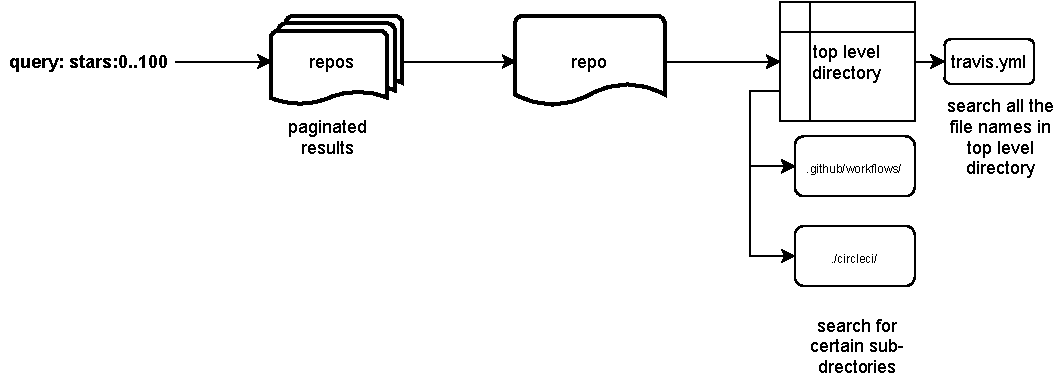
\includegraphics[width=\textwidth]{methadology diagram.pdf}
  
  \caption[alt text]{Diagram of the process used to search for projects with CI files in them}
  \label{image_methadolgoy_diagram}
\end{figure}

As can be seen in Figure \ref{image_methadolgoy_diagram} do a query based on the number of stars a project has on Github. This is because we need a way of getting a large sample from Github without introducing too much bais into the sample. That is not too say that our method is perfect but it provides an easy way to get a large sample that includes projects with and without CI.
Another potential solution would have been to use the \enquote{filename:travis.yaml} search api. However this did not provide information about which projects did not use CI. As well as for one unique search their can only be 1000 results returned by the Github Api. To mitigate that limit we search based stars as we did do a search for a 1000 results per star count. The limitation of this though was that there will be over a 1000 repositories that have 0 to 500 or even 500 to 501 stars. That means it is a sample that represents some of the population not a sample of all CI files on Github. 

As the config could have mistakes in it or we missed out a major CI system. We also saved the ReadMe.md when we scraped each project. A Readme.md is used to describe a project and will be displayed on Github at the bottom of the root directory. As can be seen in Figure \ref{ExampleGithubReadme} some ReadMe's have a label and/or links to the CI system used for that project. Therefore we also save that data when we scrape a project. 

\begin{figure}[h]
  \centering
  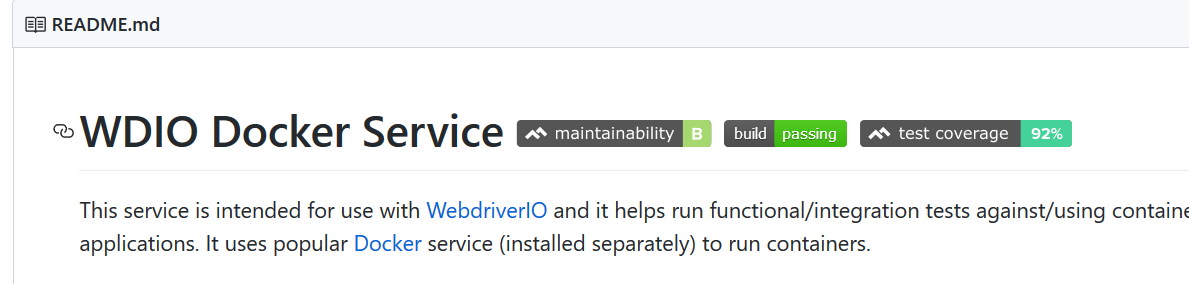
\includegraphics[scale=0.5, width=\textwidth]{2020-01-30-08-29-04.png}
  
  \caption[alt text]{Example of CI tag for Github ReadMe \cite{GithubReadMeExample}}
  \label{ExampleGithubReadme}
\end{figure}

We ended up with a config file with queries for configuration files for the following CI systems: Travis, Gitlab, Azure, App Veyor, Drone, Jenkins, Github, Circleci, Semaphore, Teamcity and Buildkite. 

We excluded Wrecker from the search because they represented a very small number of projects in comparison to the other projects. As it seems since the Github survey in 2017 they got bought by Oracle and from doing a search on Github for what we think based on the docs \cite{WreckerDocs} and \cite{WreckerOpenSourceGithubSearch} for their config file naming convention. We were only able to find 20 results so did not include in the scraping script to speed up the process of searching for the other configuration file formats.

Along with information of what CI is being used for a project we also gathered metadata about the project. The available metadata through the api is largely what can been seen on a repository for example in Figure \ref{ExampleGithubMetaData}. We have the star count which is an indication how popular a project is as users can star projects that they like \citet{Borges2016}. Then we have watchers which is users that have subscribed to the project to get notifications about the project. 

\begin{figure}[h]
  \centering
  \includegraphics[scale=0.5, width=\textwidth]{readme metadata example.png}
  \caption[alt text]{Example Github project description and metadata\cite{GithubMetaDataExample}. The orange sections sections highlighted are the metadata that we scraped.}
  \label{ExampleGithubMetaData}
\end{figure}

\vspace*{-0.05in}
\subsection{Data corpus}
\label{section:corpus}
\vspace*{-0.05in}
This all produced a sample of 32,660 projects from open source projects on Github. As can be seen in Figure \ref{graph_scatter_stars_vs_subs} we weren't able to scrape the whole star count range easily. This is because the script would crash when Github gave a 500 error code at us randomly. Along with empty repositories initially causing a problem. In order to mitigate the damage of this the scraper would create a new Comma Separated Value (csv) file search e.g. one for stars:0..1 and another for stars:1..2. As all the csv file contained the same header we ran a script to combine all together at the end. Making sure to remove any duplicates by filtering on the Github project id.

\begin{figure}[!htbp]
  \centering
  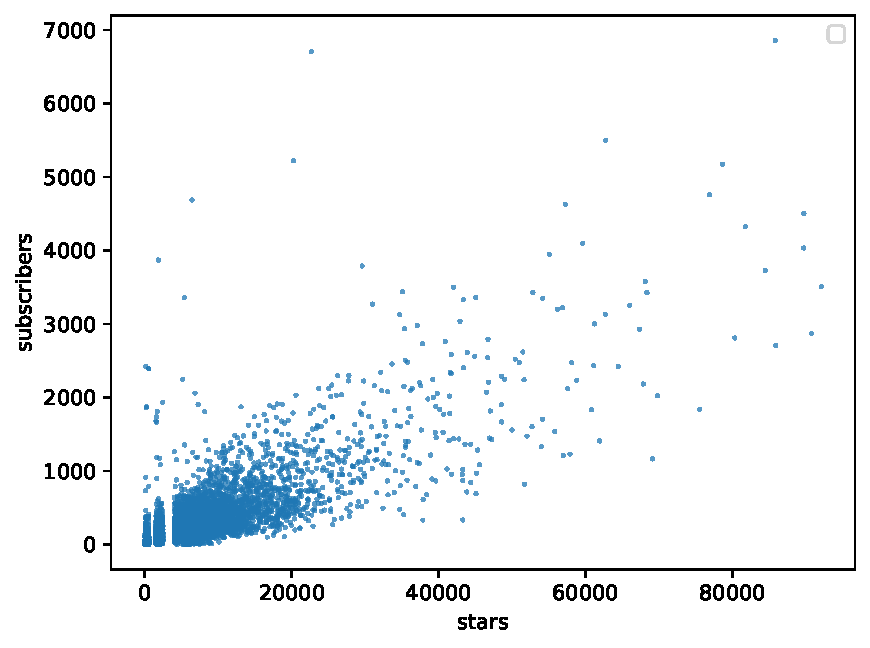
\includegraphics[width=\textwidth]{../src/results/sub vs stars.pdf}
  \caption[alt text]{Github stars against subscribers}
  \label{graph_scatter_stars_vs_subs}
\end{figure}

\vspace*{-0.05in}
\subsection{Comparison corpus info}
\label{section:HiltonComaprisonCoprusTHing}
\vspace*{-0.05in}
In \citet{Hilton2016} paper they use a similar method of using the Github Api in order to create their corpus. Additionally they contacted Cloud Bees \citet{CloudBees2020} to get a list of all open source projects that used their services. This helped them not to miss out on projects that they would otherwise missed out on. They kindly gave a copy of their final corpus. 

However it does contain the data on the Cloud Bees projects which is 223 projects. As far as we can tell this only effects the comparison done in RQ2 \ref{section:RQ2}. Additionally we found slight discrepancies between the paper and corpus in RQ1, RQ2 and RQ3 mainly just a few numbers off in a few places. In order to do comparisons well and to keep it consistent we will be basing all our comparisons from the corpus. As the discrepancies are small we will using the conclusions from the paper where possible.  

In order to get a better understanding of the results of the methodologies chosen in both cases. We created Figure \ref{graph:hist} two histograms to showing the density by the stars of the spread of data using the Sturge's rule. As we expected both corpses are skewed to the left.  

\begin{figure}[!htbp]
  \centering
  \begin{minipage}{.48\textwidth}
    \centering
    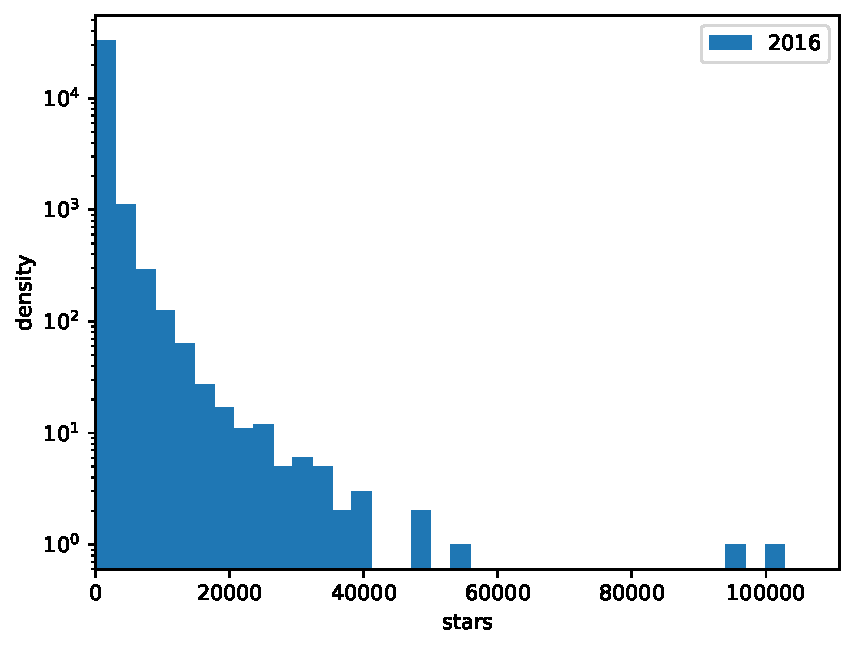
\includegraphics[width=\textwidth]{../src/results/density_2016.pdf}
    \caption[]{2016 corpus}
    \label{graph:hist2016}
  \end{minipage}
  \begin{minipage}{.48\textwidth}
    \centering
  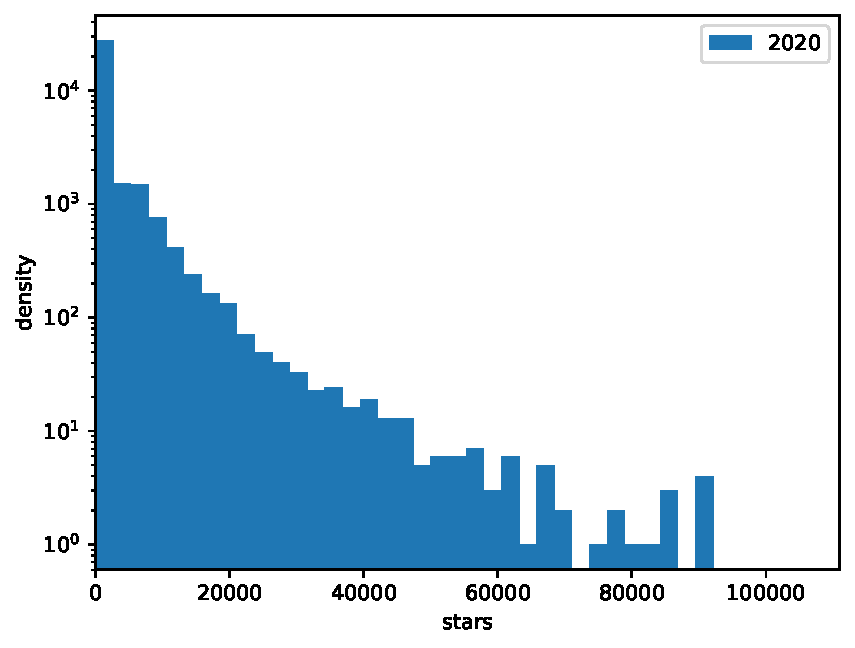
\includegraphics[width=\textwidth]{../src/results/density_2020.pdf}
  \caption[]{2020 corpus}
  \label{graph:hist2020}
  \end{minipage}
  \caption[]{Histogram showing the density for both corpses via the stars of the projects. They are both skewed towards to the lower star count projects. }
  \label{graph:hist}

\end{figure}
% https://www.cloudbees.com/
% ------------------------------------------------------------------------------------------------------------------------------------

\pagebreak
\section{Usage of CI}

\vspace*{-0.05in}
\subsection{\textbf{RQ1}: What percentage of open-source projects use CI?}
\label{section:RQ1}
\vspace*{-0.05in}

Out of the 31,752 projects 38.39\% of them had CI configuration files in them indicating that they used CI in our dataset. 

\begin{table}[!ht]
    \begin{tabular}{l|l|l|l|l|}
    \cline{2-5}
                                                & \multicolumn{2}{c|}{\textbf{2016}} & \multicolumn{2}{c|}{\textbf{2020}} \\ \cline{2-5} 
                                                & count         & percentage         & count         & percentage         \\ \hline
    \multicolumn{1}{|l|}{\textbf{Found CI}}          & 13752         & 39.81\%            & 12538         & 38.39\%            \\ \hline
    \multicolumn{1}{|l|}{\textbf{No CI found}}       & 20792         & 60.19\%            & 19214         & 58.38\%            \\ \hline
    \multicolumn{1}{|l|}{\textbf{ReadMe has CI status}}      & \multicolumn{2}{c|}{n/a}           & 908           & 2.78\%             \\ \hline
    \multicolumn{1}{|l|}{\textbf{Total}}      & \multicolumn{2}{c|}{34,544}           & \multicolumn{2}{c|}{31,494}             \\ \hline
    \multicolumn{1}{|l|}{\textbf{Multiple CI}} & 1796          & 12.91\%            & 1764          & 14.07\%            \\ \hline

    \end{tabular}
    \label{table:comparison_dataset}

    \caption{This table shows the comparison between the 2016 dataset which is\citet{Hilton2016} and our dataset labeled as 2020. For the CI usage in each dataset along with what percentage of projects contained multiple CI setups.}
\end{table}
% table references are not working because the table was being rendered below the reference.... ah! but it's fixed atm 
An interesting factor in Table \ref{table:comparison_dataset} is the percentage of that 38\% that has multiple CI in them. This is because configuration files can be used to CI or CD and some projects are run a monorepo which means that have multiple projects inside them. Another simple explanation is that although the configuration is stored version control it just hasn't been deleted. 

We scraped the \enquote{ReadMe.md} files from the projects to check if they had a CI status label in them as shown in Figure \ref{ExampleGithubReadme}. To do this we checked for \verb|alt="Build Status"|, \verb|alt=`Build Status'|, \verb|Status| and \verb|status| being in the file. Then if that same line of text contained a url specified by if contained \verb|http://| or \verb|https://| then we counted it as potentially being a project that used CI. In order to check the validity of this method we ran it on all projects that we had found configuration files for. We got 6782 (55.92\%) projects with a ReadMe that had a CI status label that we could find.
However this method is not perfect, for example \enquote{awesome-bootstrap-checkbox} by \enquote{flatlogic} \cite{GithubReadMeIncorrectFind} there ReadMe has the following line:
\begin{verbatim}
  [![Dependency Status]
  (https://img.shields.io/david/dev/flatlogic/awesome-bootstrap-checkbox.svg?branch=master&style=flat)
  ]
  (https://www.npmjs.com/package/awesome-bootstrap-checkbox) 
\end{verbatim}
This contains \verb|Status| and a url so we say it has got CI when the repository currently doesn't. Yet this is not the case for all of them as for example \enquote{SyncTrayzor} by \enquote{canton7} \cite{Male2020} uses AppVeyor but doesn't use a configuration file for it. Therefore we didn't find it as we searched for a config file only. 

The percentage of CI projects they had was 39.81\%. If you look at Table 1 it shows that we got 38.51\% CI projects. This is interesting as we searched for more kinds of CI configuration so there was a potentially a higher chance of having CI.

One possible reason could be because of in RQ3 \ref{section:RQ3} it shows that the more popular a project the higher chance it has of using CI. Therefore as their sample contains a few more projects that are popular their they could all be using CI. However that is a weak tangent to make in order to full explain it.  

Another possible reason could be if you combined the \enquote{Found CI} and \enquote{ReadMe has CI status} results together for 2020 you would get 41.28\% which is shows that our sample is within the margins of the same results that of CI usage for 2016.

Another possible reason is that because of Github's growth over the last 4 years (\citet{GithubOctoverseResults2016} to 2019 \citet{GithubOctoverseResults}) so that Github is now at 40 million active users. It means that there are more projects that are using CD setups for building their static sites and in general Github is being used for more things that wouldn't require CI.

Therefore we think that the last two factors are the most likely contributors to why there is less CI usage now. Another important interesting part is despite Github growing so much the CI usage rate has stayed relatively the same. 



% --------------------------------------------------------------
\vspace*{-0.05in}
\subsection{\textbf{RQ2}: What CI systems are projects using?}
\label{section:RQ2}
\vspace*{-0.05in}
In Table \ref{table_config_types} we find like all other research Travis is the most popular CI system in use. However over the last 4 years since the \cite{Github2017} CircleCi has lost out on it's rough quarter that it owned. In particular the rise of Github Actions seems to have taken second place even though it is still very young in comparison as it was officially released November 13th 2019 but had a closed beta since the summer of 2019. However this might not be down to the CircleCi loosing out on their existing share. But potentially as the rise in CI usage goes up on Github. Projects are more likely to pick in the built in solutions to Github.
\begin {table}[!htbp]

\caption{Configuration types spread}
\label{table_config_types}
\begin{tabular}{lrl}
\hline
{} &  config & percentage \\ \hline

Travis          &   10607 &        74\% \\ \hline
Github          &    2301 &        16\% \\ \hline
CircleCi        &    1109 &         8\% \\ \hline
Jenkins pipeline &     161 &         1\% \\ \hline
Drone           &      84 &         1\% \\ \hline
Buildkite       &      32 &         0\% \\ \hline
Teamcity        &       4 &         0\% \\ \hline
Semaphore       &       2 &         0\% \\ \hline
Azure pipeline           &       1 &         0\% \\ \hline

\end{tabular}
\end{table}


\begin{figure}[!htbp]
  \centering
  \begin{minipage}{.48\textwidth}
    \centering
    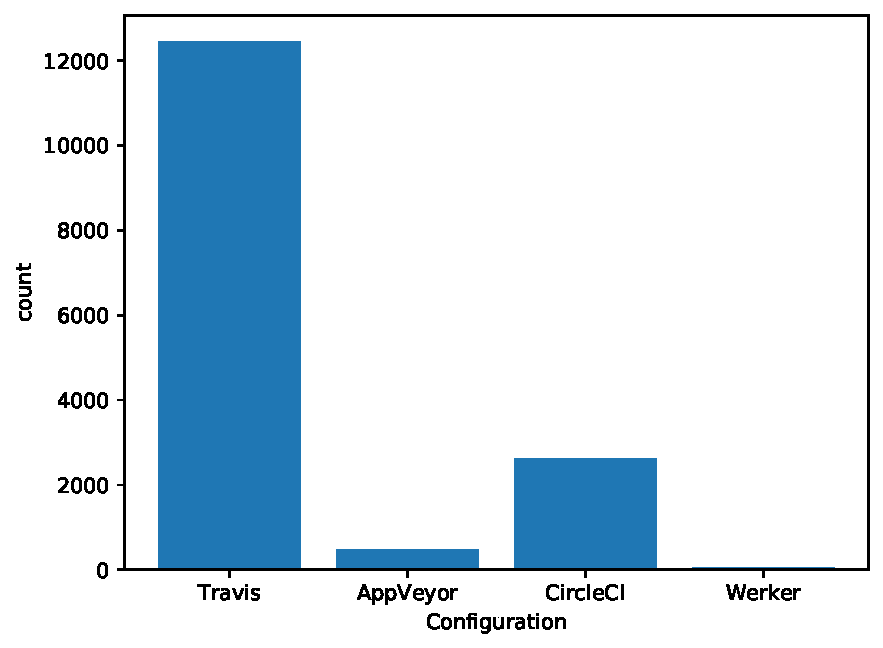
\includegraphics[width=\textwidth]{../src/results/comparison_config_bar.pdf}
    \caption[]{2016 corpus}
    \label{graph:config_bar2016}
  \end{minipage}
  \begin{minipage}{.48\textwidth}
    \centering
  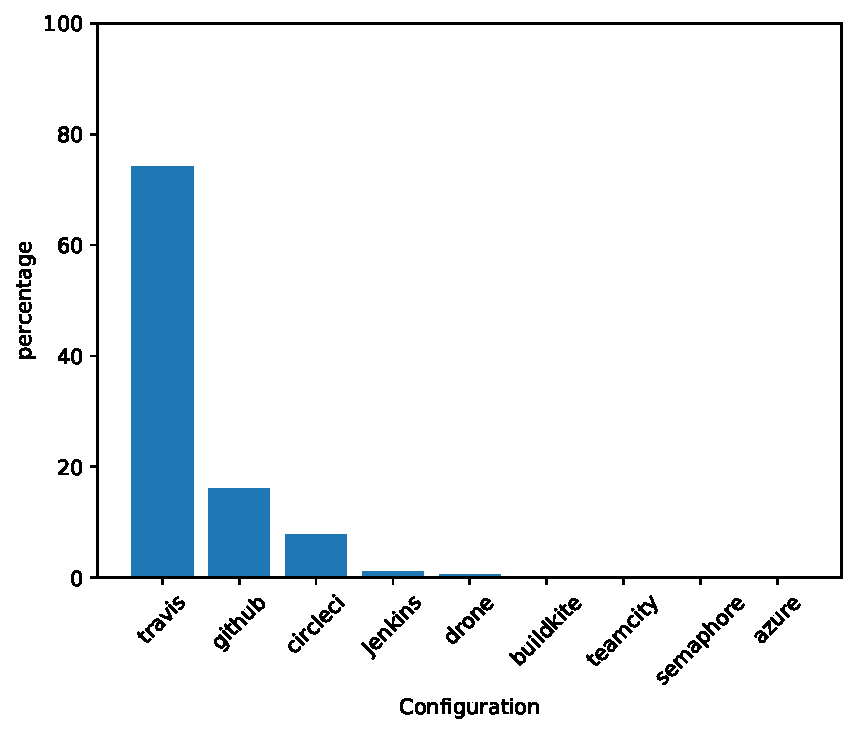
\includegraphics[width=\textwidth]{../src/results/config-topn.pdf}
  \caption[]{2020 corpus}
  \label{graph:config_bar2020}
  \end{minipage}
  \caption[]{Percentage bar graph showing the usage of each CI service. The key difference is how CircleCI has got a lower rank. Due to rise of Github Actions which only open to closed beta in August 2019}
  \label{graph:config_bars}

\end{figure}


Our sample of repositories is 31,494 this means that as it is a representation of projects on Github so won't account for the whole of it. This means that although Wrecker had the smallest count of CI when researching of 20 projects. In Table \ref{table_config_types} we have configuration types that have lower counts. This is because that search for the 20 searched the whole of Github but the scraping was only able to do a small sample. Additionally their potentially could be faults in the scraping causing it show such low numbers for the last 3. 

% ------------------------------------------------------------------------------------------------------------------------------------
\vspace*{-0.05in}
\subsection{\textbf{RQ3}: Do certain types of projects use CI more than others?}  
\label{section:RQ3}
\vspace*{-0.05in}

Below shows all the CI projects sorted then grouped together per 540 projects. Then in this case we choose to categories via star count for each project. 

\begin{figure}[!htbp]
  \centering
  \begin{minipage}{.48\textwidth}
    \centering
    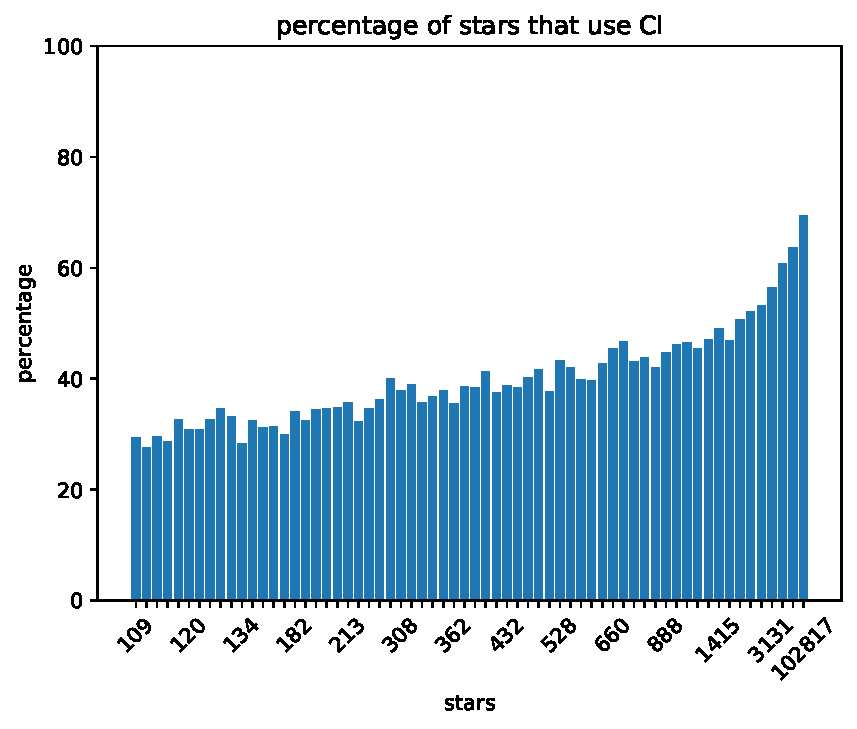
\includegraphics[width=.9\textwidth]{../src/results/percentage sub with CI other paper source.pdf}
    \caption[]{2016 dataset}
    \label{fig:test2}
  \end{minipage}
  \begin{minipage}{.48\textwidth}
    \centering
    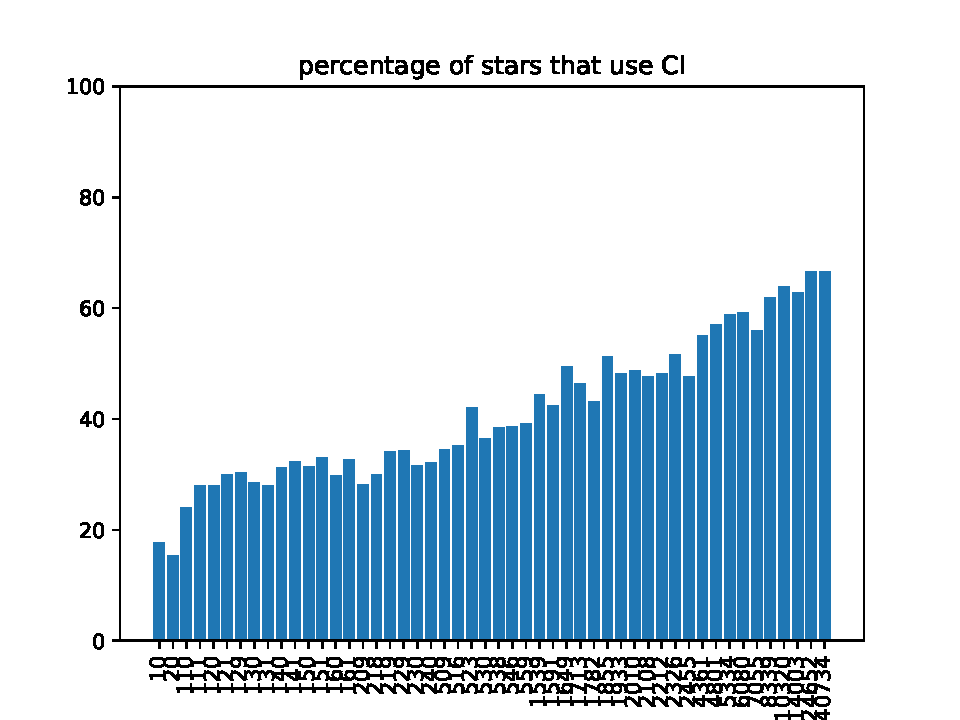
\includegraphics[width=.9\textwidth]{../src/results/percentage stars with CI.pdf}
    \caption{2020 dataset}
    \label{fig:test1}
  \end{minipage}%
  \hfill
  \caption{In Figure \ref{fig:test1} is the results from this research and in Figure \ref{fig:test2} is the results from \cite{Hilton2016}. The results show the percentage chance of CI usage depending on the number of stars a group of 540 projects has on average.}
  \label{fig:comparison_percentage_star_usage}
\end{figure}

Here in Figure \ref{fig:test1} and \ref{fig:test2} we are comparing whether or not in the last 4 years the number of stars increases the CI being used. It shows how the trend in the more popular the project by how you have more stars for a project increases the chances it uses CI has stayed the same. However the gradient of that trend has changed to be slightly greater overall. Yet not quite as sharp for the end of the graph this is most likely because the 2016 dataset doesn't have as much data between 40000 and 90000 as seen in Figure \ref{graph:hist2016}.

\begin{figure}[!h]
  \centering
  % TODO: make this bigger when the time comes
  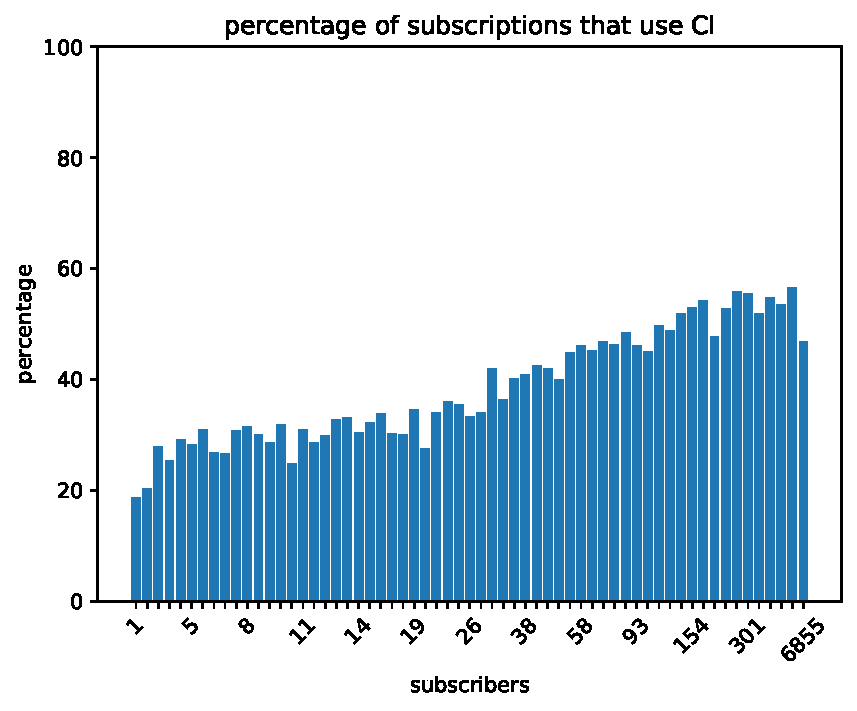
\includegraphics[width=.8\textwidth]{../src/results/percentage sub with CI.pdf}
  \caption{Subs graph}
  \label{graph_percentage_subs}
\end{figure}
Figure \ref{graph_percentage_subs} uses the same method as Figure \ref{fig:comparison_percentage_star_usage} except is does it based the number of subscribers. Subscribers are used on Github to keep update on the changes on the project. This could range from core team members working on the project to people that want to be notified about a new release. 
In looking at this metric the hypothesis was that it would have a sharper rise in percentage of projects using CI per subscriber. However that was not the case overall the gradient is not as strong. There is no comparison to \cite{Hilton2016} because their final corpus does not contain subscriber count for each project.

That gives us a good look at how projects can be viewed through Github's metadata. 


In terms of what kind of programming languages are being used for CI? As well as what programming languages where found when creating the sample. We can see the top 20 results in Figure \ref{graph:programming_langs_count_ci} in that we can see that Javascript is the most common kind of project. This was too be expected as in Github's annual report \cite{GithubOctoverseResults} on the platform they reported that Javascript has been the most popular for the last 5 years. The interesting part is that our sample matches the rise in Python over Java. Despite the fact that they are using \enquote{unique contributors to public and private repositories tagged with the appropriate primary language} and we are using the count of projects by primary programming language tag. 

\begin{figure}[!h]
  \centering
  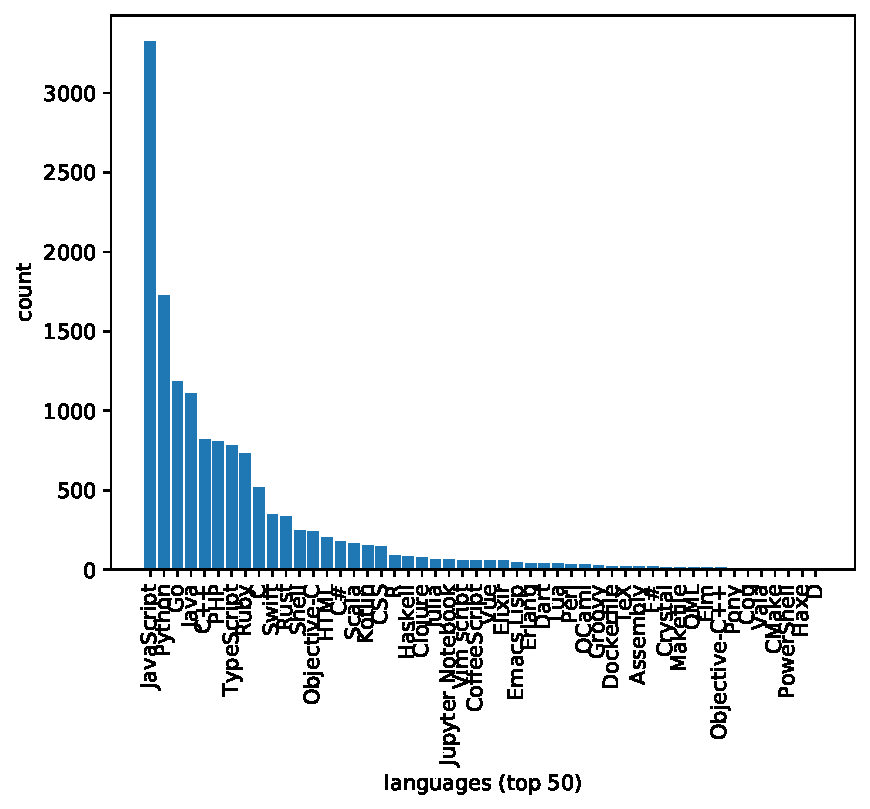
\includegraphics[width=.8\textwidth]{../src/results/languages-topn.pdf}
  \caption{Count of top 20 programming languages used by projects using CI}
  \label{graph:programming_langs_count_ci}
\end{figure}

In order to get a better idea of the breakdown of the effect programming languages have on CI usages. We created Figure \ref{graph:scatter_langauges_CI} this shows three peices of information the percentage of CI usage on the y axis, average star count on the x axis and then number of projects using the language by the size of the dot. 

\begin{figure}[!h]
  \centering
  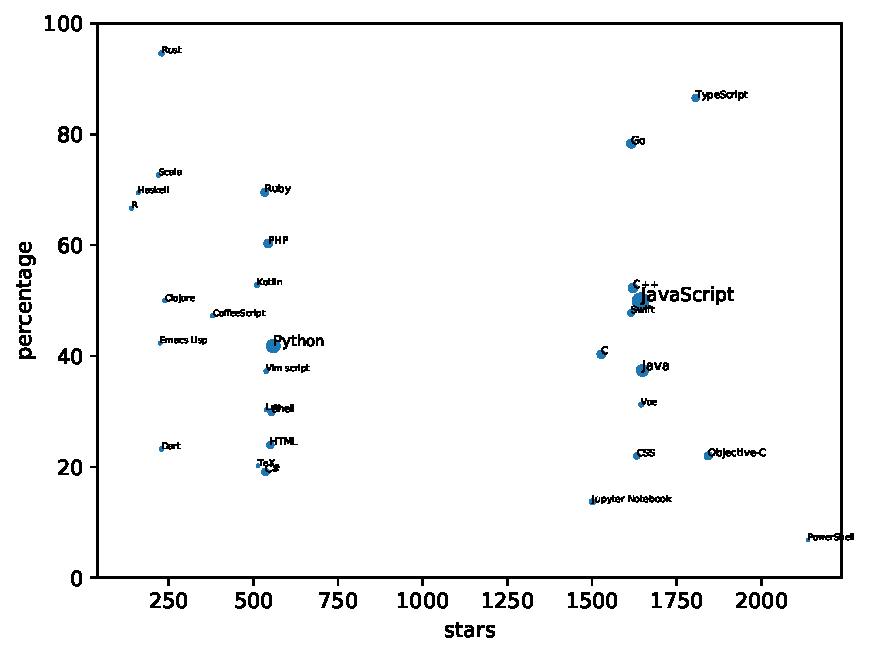
\includegraphics[width=.8\textwidth]{../src/results/languages-scatter-CI.pdf}
  \caption{Scatter graph showing the top 30 most used programming languages against how much they use CI. The key points are Rust, Typescript and Go being the top three programming in CI usage.}
  \label{graph:scatter_langauges_CI}
\end{figure}


The most striking part of Figure \ref{graph:scatter_langauges_CI} is the clear divide between different programing languages star count. The programming with the languages with the highest CI usage are Rust (94.6\%), Typescript (86.56\%) and Go (78.31\%). This is interesting in how they are all fairly \enquote{new programming languages} in comparison to the others in the graph. They are all languages which are developed and open source on Github. In terms of Rust and Go it could be down to their tooling that comes builtin to the language. As that would lead to implementing CI to be a lot easier. Yet Typescript is more a special case as it is a subset of Javascript so uses `npm' to deal with dependency management which was some of inspiration for Rust's tooling \citet{RustBlogCargo}. Older programming languages like Java and C\# both have tooling for dependency management but the chances that they use CI is much lower. Therefore an area for further research would be whether or not the use \enquote{modern} dependency management systems increases the chance of CI.

\begin{figure}[!h]
  \centering
  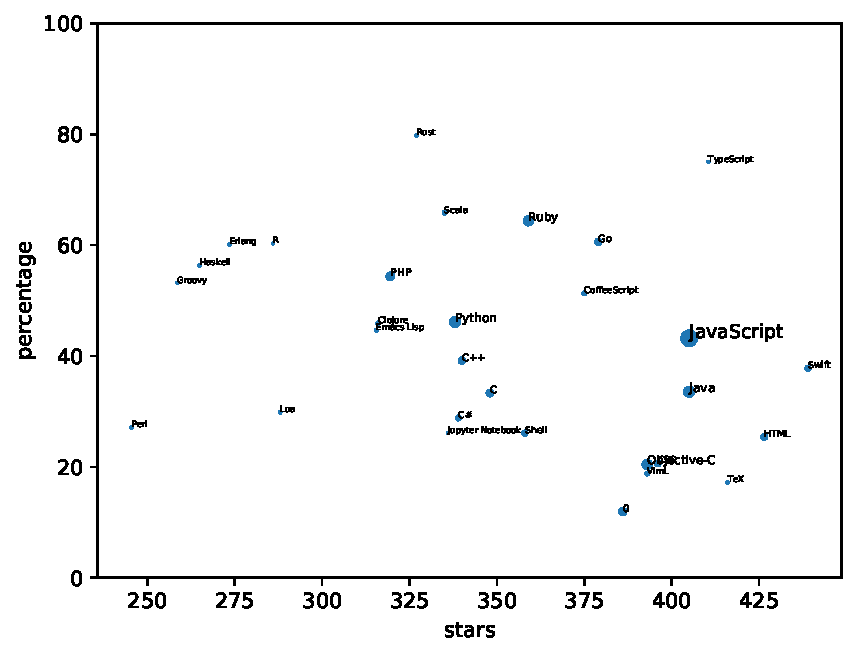
\includegraphics[width=.8\textwidth]{../src/results/scatter.pdf}
  \caption{Scatter graph showing the top 30 most used programming languages against how much they use CI for \citet{Hilton2016} from 2016. In comparison to Figure \ref{graph:scatter_langauges_CI} the data is not as grouped as clearly by the star count. Rust, Typescript and then Scala have the highest programming CI usage.}
  \label{graph:scatter_langauges_CI_2016}
\end{figure}

In figure \ref{graph:scatter_langauges_CI_2016} it shows the sample from 2016 in comparison to \ref{graph:scatter_langauges_CI}. The first major difference is in how the spread languages by stars isn't as divided. This could be because of how the sample is not as spread out as seen in Figure \ref{graph:hist}. The scatter graph is for the top 30 most common programming languages found from this Rust, Typescript and Scalar have the highest chance of using CI. This is really interesting is that Rust and Typescript are still really within the top 3 after 4 years. Potentially this could be to do with the ecosystem around the languages that lead this. However this an area for further research of why different languages have a higher chance of using CI. 

Finally one observation that was made in \citet{Hilton2016} paper was that their was a higher chance of CI usage for dynamically typed languages. We looked into analysing this as we found both Rust and Typescript having really high CI usage chance. Yet at the same time overall Javascript and Python had the most projects that used CI. So we wanted to look at where the balance lied in the difference between the two. However categorising the programming languages by their usage is difficult. For example is a Javascript a project that is using Typescript's js checking dynamically typed or statically typed? And then how do you tell? Or if you have a similar situation where Python has static types. Therefore this an area for further research as it is a question that would need to carefully answered.

Overall popularity of the project increases the chances of it using CI. The programming language has effects the chances of it using CI. However what properties of the language cause this effect is unclear so is an area for further research.

% \begin{figure}[!h]
%   \centering
%   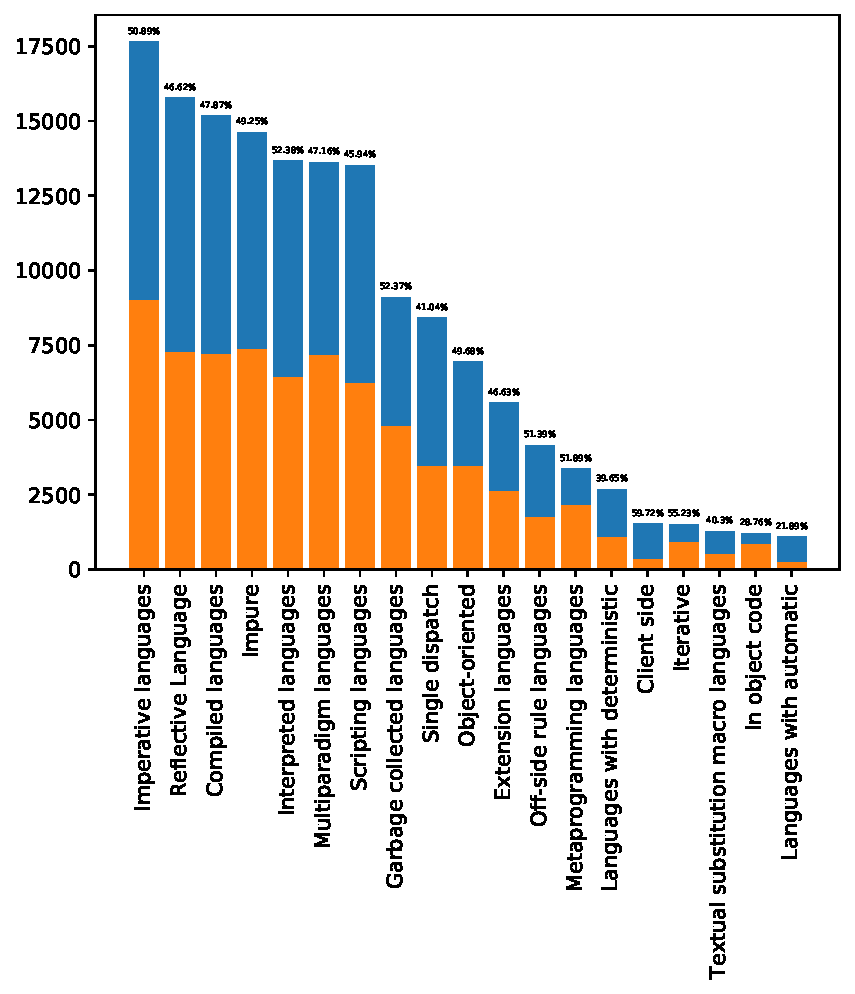
\includegraphics[width=.8\textwidth]{../src/results/languages.pdf}
%   \caption{Using categories found on Wikipeada \citet{2020Wiki} we categorised what kind of programming languages used CI. The key factor is the difference how their our more Interpreted language usage vs Compiled languages. We only included the top 20 categories of programming language.}
%   \label{graph:langs}
% \end{figure}

% We found that their is a higher chance that popular projects use CI along with those that have more subscribers to their project. In terms programming language the usage of type system contributed to a slight increase in the chance for the project. Yet it seemed there is area for further research in how the dependency and tooling effects the chances of CI being used. 
 
\pagebreak
% ------------------------------------------------------------------------------------------------------------------------------------
\section{Structure of configuration files}

The following three research questions will just be on the 14,302 CI projects (found CI plus multiple CI \ref{table:comparison_dataset}). In order to be able to ask the questions about the data we filter the sample to only include CI projects. Then we created a csv table with a row per CI type in that project as some projects had multiple versions of CI as shown in \ref{section:RQ1}. Then we processed each CI file to get the necessary data to be able to ask questions about it's structure. As we wanted to be able to process files with or without errors in along with all types of CI. We created a parser to go through each line of the configuration file working out what that line is. For example is it a comment or blank line or does it have code. 

% a little bit like running cloc on the code base

\vspace*{-0.05in}
\subsection{\textbf{RQ4}: What are the common errors when loading yaml configuration?}
\label{section:RQ4}
\vspace*{-0.05in}
Here our the 
\begin{figure}[!h]
  \centering
  \begin{minipage}[t]{.48\textwidth}
    \textbf{Scanner error}
    The first step of loading the yaml is to scan it to create the tokens. However for example tabs are not allowed in yaml \citet{YAML_FAQ_TABS} as seen in the example with \enquote{\textbackslash t} representing a tab. 
  \end{minipage}%
  \hfill
  \begin{minipage}[t]{.48\textwidth}
    \begin{verbatim}
      definitions: 
      \t- build
    \end{verbatim}
  \end{minipage}
\end{figure}
\begin{figure}[!ht]
  \centering
  \begin{minipage}[t]{.48\textwidth}
    \textbf{Parse error}
    In this example it has scanned the file and created tokens for the syntax. Now it parses the syntax and works out if each token is valid given it's current context. In this case a closing \verb|]| without an opening \verb|[| is invalid.
  \end{minipage}%
  \hfill
  \begin{minipage}[t]{.48\textwidth}
    \begin{verbatim}
      definitions: ]
    \end{verbatim}
  \end{minipage}
\end{figure}

\begin{figure}[!ht]
  \centering
  \begin{minipage}[t]{.48\textwidth}
    \textbf{Composer error}
    In the example it has two steps that are using an yaml anchor. This allows for the yaml to be referenced somewhere else. However if you define the anchor twice with the same name it causes an composer error. As you have two references using the same name so it won't know which one to use.
  \end{minipage}%
  \hfill
  \begin{minipage}[t]{.48\textwidth}
    \begin{verbatim}
      definitions: 
      steps:
      - step: &build-test
      name: Build and test
      script:
      - mvn package
      - step: &build-test
      name: deploy
      script:
      - ./deploy.sh target/my-app.jar
    \end{verbatim}
  \end{minipage}
\end{figure}



\begin {table}[!htbp]

\caption{cats}
\begin{tabular}{|l|l|l|l|}
\hline
\textbf{yaml\_encoding\_error} &  composer error &  parse error &  scanner error \\ \hline
\textbf{config  } &                 &              &                \\ \hline

\textbf{circleci} &               0 &            0 &              1 \\ \hline
\textbf{drone   } &              30 &            0 &              0 \\ \hline
\textbf{github  } &               0 &            0 &              3 \\ \hline
\textbf{travis  } &               6 &           10 &             21 \\ \hline

\end{tabular}
\end{table}

As can be seen in the Table \ref{table_yaml_errors} their our configuration files with yaml errors meaning that the CI for that project will not load correctly. Yet it seems that a very small percentage of projects that have them. For example the two highest configuration types with errors are Drone (36.90\%) followed by Travis (0.348\%).

In the case for Drone all the errors are for the same type of error. Potentially this could be because of how anchors are a lot more common in Drone.

For Travis as it is the largest config type out of the sample by a significant amount it is more likely to contain more errors. Yet with such a small amount it seems like yaml errors aren't a major problem in CI. Although as they are required to be fixed in order for the CI to run the chances are the ones with errors ones that are being changed when the scraping was being done. Meaning that as the CI has been set up correctly for the other 99.632\% as they are not needing to change because their our no yaml errors in it and presumably it is doing what they intend for it to do.


\pagebreak
% -----------------------------------------------------------------
\begin{figure}[!ht]
  \vspace*{-0.05in}
  \subsection{\textbf{RQ5}: How are comments used in configuration?}
  \label{section:RQ5}
  \vspace*{-0.05in}
\end{figure}


The assumption was the as continuous integration setups can be complicated and have edge cases. Therefore comments would be used to describe and handle that complexity.

An example configuration file below for Github actions using the default template slightly altered. Shows two examples of comment usage, the first being including useful information about why a particular version of the programming language was chosen. The second is that the tests have been disabled by commenting them out. 



\begin{figure}[!htbp]
  \centering
  \begin{minipage}[t]{.48\textwidth}
    In order to pick up on all these different types of comments. All the CI files were parsed and then regular expressions were used to pick on up key factors such as "note:". Along with multiple single line comments which made up a block/multi-line comment.
    
    For example in to the left there is an example Github Action yaml file. If were it would be parsed we would get: one multi line comment, 15 lines of code, 1 single line comment, a total of 5 comments and 20 lines in the file. Therefore their is a their is a ratio of 4:1 for code in this config file.
  \end{minipage}%
  \hfill
  \begin{minipage}[t]{.48\textwidth}
    \begin{verbatim}
      name: Python package
      on: [push]
      jobs:
      build:
      runs-on: ubuntu-latest
      steps:
      - uses: actions/checkout@v2
      - name: Set up Python
      uses: actions/setup-python@v1
      # note: only works with python 3
      with:
      python-version: 3.8
      - name: Install dependencies
      run: |
      python -m pip install --upgrade pip
      pip install -r requirements.txt
      #      - name: Test with pytest
      #        run: |
      #          pip install pytest
      #          pytest ./src
    \end{verbatim}
  \end{minipage}
\end{figure}

% NOTE: NEED TO EXPLAIN CODE_WITH_COMMENTS

Initially before we look at the comments it is important to understand how the rest of the file is made up. In the graph below (Figure \ref{fig:bar_comments_lines}) it shows how each configuration type is made up by mean of each part of the file. For all the yaml based configurations lines of code and number of lines in total are very close. Then for the number of comments being very very small on average.

In the case for Jenkins pipelines and Teamcity there is a much higher usage of having code with comments. 


\begin{figure}[!ht]
  \centering
  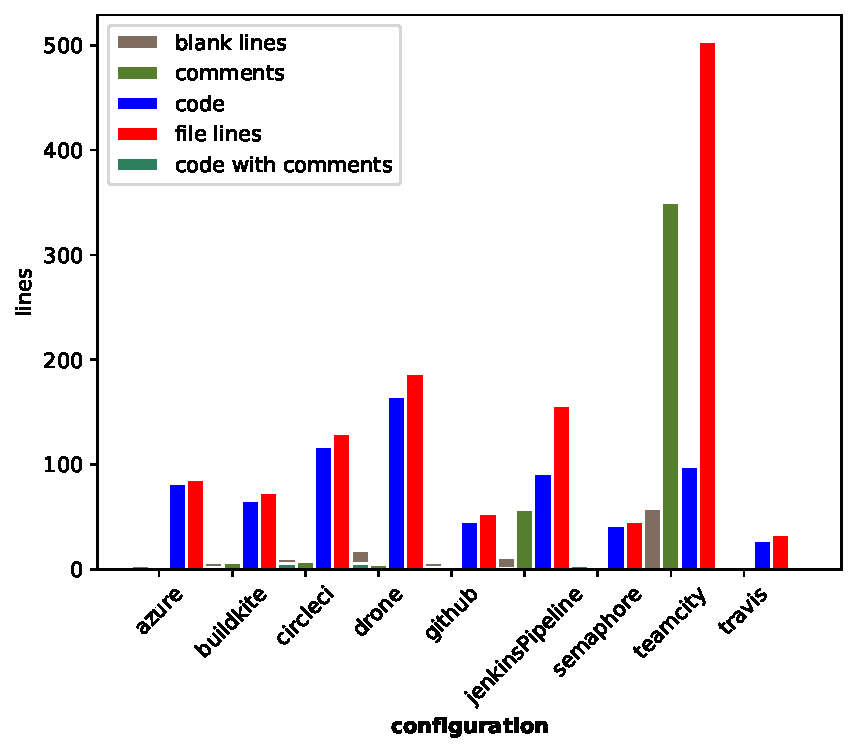
\includegraphics[width=\textwidth]{../src/results/basic comments bars.pdf}
  \caption[alt text]{Mean of line counts}
  \label{fig:bar_comments_lines}
\end{figure}

% plan:
% - grouped bar chart for blank lines, comments, code, file lines (with a zoomed in version and splitting up of yaml and non yaml)
% 
% comment bars: single, multi and code (which is kind of like the zoomed in )
% this will give us a representation of the median which will allow us to discuss and expalin everythign clearly. And hopefully be eaisly visinbble!!
% 




% so we are not going to do raitos as they don't work for what we are wanting to do
% as well as they are really compilcated to do well. As in you have:
% 
% config:
%   - file
%     - file lines
%     - blank lines
%     - code
%     - multiple types of comments
% 
% so in order to work out the raito you can do it per file easily -ish (as you can have comments and code...)
% 
% 
% Ratios:
% \begin{itemize}
%   \item{code: comments}
%   \item{code: line total}
%   \item{code: blank lines}
%   \item{single line comment: multiline comment}
%   \item{single line comment: code with comment} 
% \end{itemize}






\begin{figure}[!ht]
  \centering
  \begin{minipage}[!t]{.48\textwidth}
    In Figure \ref{fig:comment_types} a regular expression was used to label the comments. There were key different types of comment that we wanted to find. The first being the commented out code which we did by searching for version numbers in commments. The second being useful information about the structure of the CI file such todo, note, importanat comments (e.g. //todo). In order to increase the search for this we included searching for urls and seperation comments (e.g. //===).
    
  \end{minipage}%
  \hfill
  \begin{minipage}[!t]{.48\textwidth}
    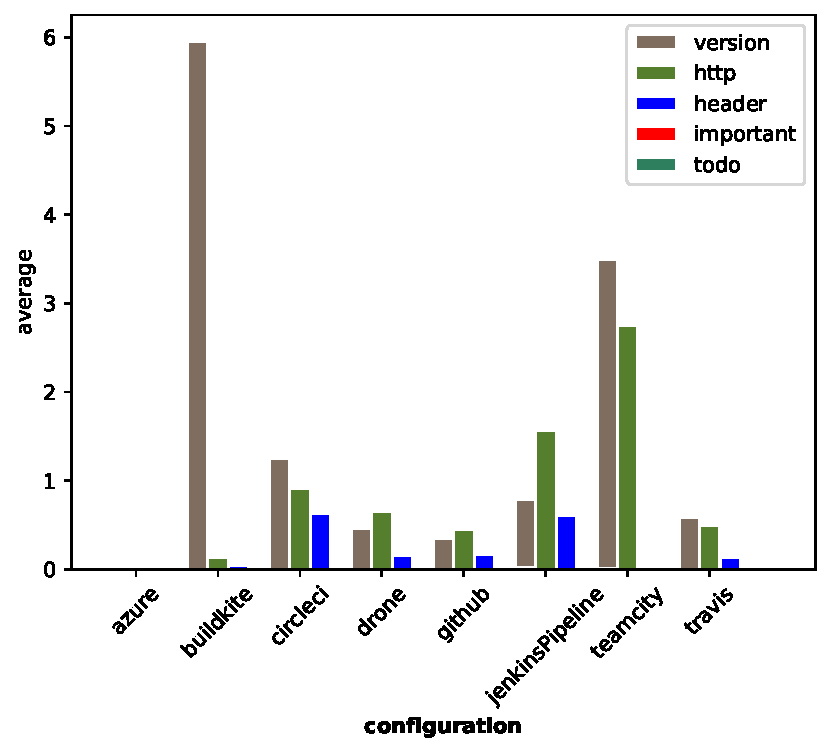
\includegraphics[width=\textwidth]{../src/results/comments usage bars.pdf}
    \caption[alt text]{Comment types}
    \label{fig:comment_types}  
  \end{minipage}
\end{figure}

From labelling the comments in Figure \ref{fig:comment_types} we can see that having comments with versions in and urls is most common. This could indicate comments from templates or how they are commented. Although yet again the amount of labels found on average is still very low.

Overall we have found that comments are not used a lot. In the cases that they are used it's more likely to be from a configuration template or commenting out configuration.
% NOTE: update this when raitos are done

\pagebreak
% ------------------------------------------------------------------------
\vspace*{-0.05in}
\subsection{\textbf{RQ6}: Are external scripts used within the configuration?}
\label{section:RQ6}
\vspace*{-0.05in}

An external script is a bash or powershell script typically depending on the operating system. It can be used to build, deploy or do any step that CI takes. The key difference between it and the CI configuration is that it be executed on a users machine. Therefore you do get some setups where you have scripts defined for building and deploying the code that the users and CI both use. Most CI systems allow for "script" tags to be used which could be described as an internal script. Therefore external scripts are defined outside the CI configuration in the directory.

The methodology we used to handle this was too look at how many bash or powershell scripts where used in CI. Using the code the parsed the yaml files for comments we were able to check do a using a regular expression for either of those files.  


\begin{figure}[!ht]
  \centering
  \begin{minipage}[!t]{.48\textwidth}
      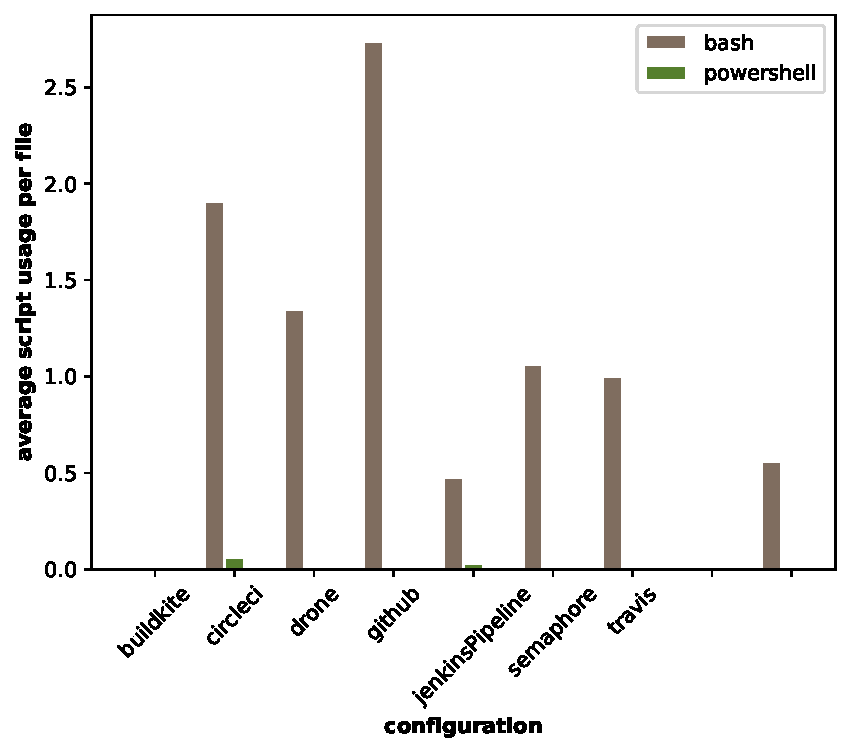
\includegraphics[width=\textwidth]{../src/results/scripts usage bars.pdf}
      \caption[alt text]{Comment types}
      \label{fig:script_usage}  
  \end{minipage}%
  \hfill
  \begin{minipage}[!t]{.48\textwidth}
    

\caption{sum of scripts used}
\label{table:scripts used}
\begin{tabular}{|l|l|l|}
\hline
{} &  bash &  powershell \\ \hline

\textbf{buildkite      } &    61 &           2 \\ \hline
\textbf{circleci       } &  1497 &           8 \\ \hline
\textbf{drone          } &   230 &           0 \\ \hline
\textbf{github         } &  1097 &          65 \\ \hline
\textbf{jenkinsPipeline} &   171 &           0 \\ \hline
\textbf{semaphore      } &     2 &           0 \\ \hline
\textbf{travis         } &  5937 &           3 \\ \hline

\end{tabular}


  \end{minipage}
\end{figure}

In Figure \ref{fig:script_usage} we have the average number of times a script is used for a configuration file that already has a script being used.

As some of the necessary actions are being done in the scripts and not in the CI file. Potentially there could be less lines of code in the configuration for files that use scripts. However in Figure \ref{fig:script_scatter_lines} we can see that the data is very spiky with outliers. Then in Figure \ref{fig:script_scatter_lines2} we can see the same affect when trying to see if the more popular a project is affects the chances of it using CI.

\begin{figure}[!ht]
  \centering
  \begin{minipage}[!t]{.48\textwidth}
    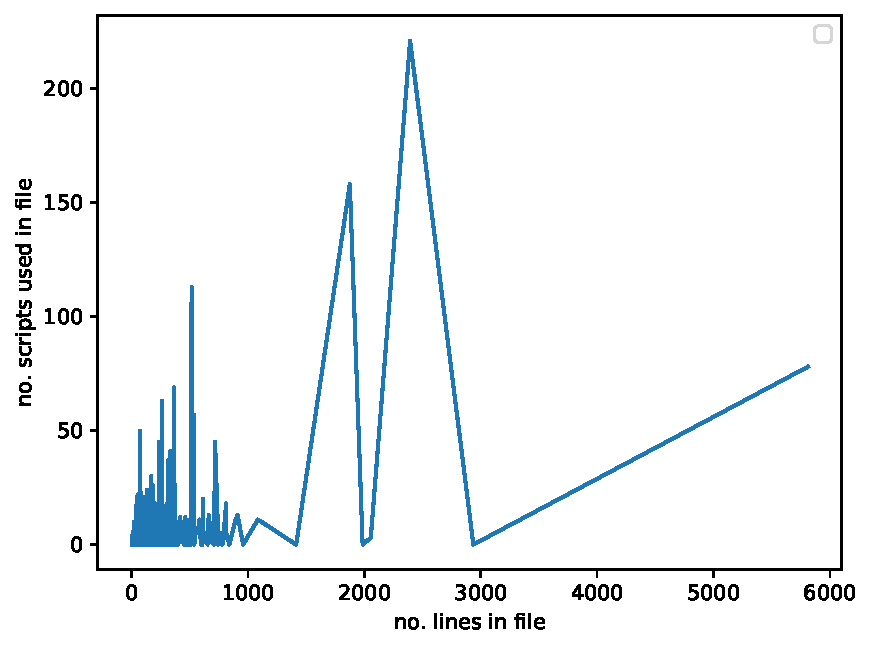
\includegraphics[width=\textwidth]{../src/results/scripts vs lines.pdf}
    \caption{no. scripts to no. lines}
    \label{fig:script_scatter_lines}    
  \end{minipage}%
  \hfill
  \begin{minipage}[!t]{.48\textwidth}
    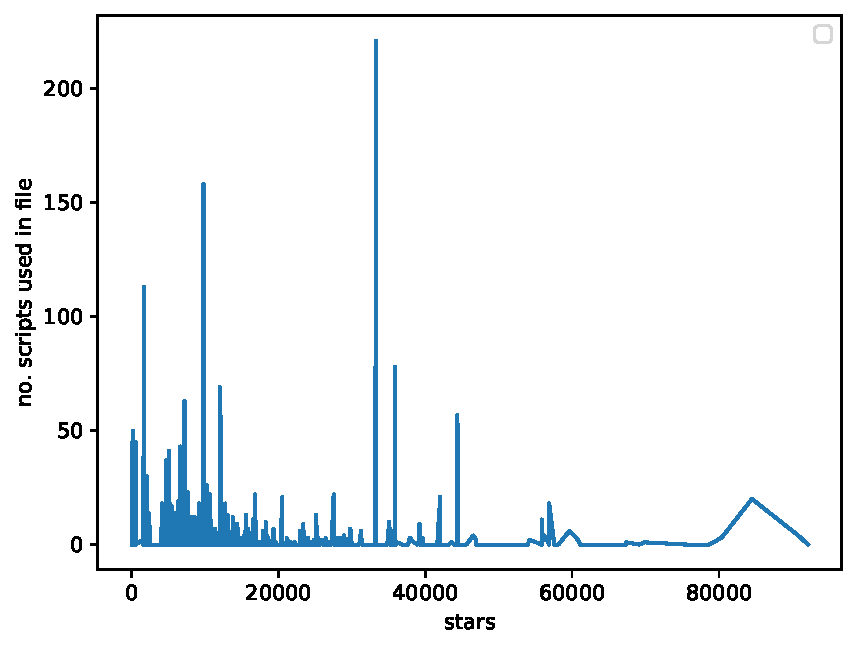
\includegraphics[width=\textwidth]{../src/results/scripts vs stars.pdf}
    \caption{no. scripts to stars}
    \label{fig:script_scatter_lines2}
  \end{minipage}
\end{figure}

\todo[]{percentage of usage needed like we had for comments}
Overall we can see that scripts are not used that much. And their no correlation between lines of code and usage of external scripts.


\pagebreak

\section{Threats to validatity}

The major and most obivious threat is the sample gathered from scraping the data from Github. This has already been touched on in the \ref{methodology} section but now we are going to look at it in more detail.

Firstly if we assume that the scraping works perfectly then it's only at maximum a 1000 open source projects per star. That is excluding closed source projects which would range from personal projects to companies. As well as it is only data from Github not from Gitlab, bitbucket or other version control hosting services. This leads to bais in the data for example if Gitlab was also scraped then we would get a lot more Gitlab ci files. However in order to get best spread of data Github has the best api and most services do not tie you down to use only their service. As well although we could get a 1000 projects per star we were still able to get around 30,000 projects and a wide spread across Github. The key aspect being that because it was a sample we focused on getting a good spread of data.

Secondly the scraping script is not perfect in how it finds configuration files. As it only looks in the top level directory for the file name pattern described in their docs or unique folder. Therefore if the systems allowed many different names or different names in past it wouldn't have picked it CI system. Additionally we only decided to scrape for certain CI files. Yet we chose a good scope based on previous research into the top CI files. As well the scraping script has been tested worked on to try and minimise any bugs. In the case that we did not pick up a CI file we ran a regexp against the ReadMe file to get a better understanding of the error bounds.

Thirdly identifying which projects are programming projects or would have a need for CI. Based on the research \cite{Kalliamvakou2014} it is important to filter out repositories that aren't part of the question being asked. Therefore we could have looked to try and filter out Github static sites and other none software based projects. However if assume a certain type of project won't be using CI then we would be introducing bais when trying to answer how CI is used. For further research better labelling of what kind of projects are which would potentially beneficial though.

% From methadolgoy to work out how to fit in:
% There are dangers in scraping data off Github in terms of assumptions to do with the population as found in \cite{Kalliamvakou2014}. Our dataset does not contain any forked repositories. But due to time constraints number of commits and frequency of recent commits has not been looked at. This would be an interesting area of further research in order to improve the quality of the sample but also to look at how that affects the frequency of CI usage.

% Additionally the assumption that all repositories are of programming projects with code in them is wrong. A number of repositories can be used for storage, experimental, academic and other things. However they to all some extent can use CI/CD for their work as a number of books were found when looking through the dataset could use CI/CD.



% strength and validaltiy section 
% - possible issues
% - baise assume in the data
% - e.g. sampling vai star
% - focusing on Github
% - problematic of scraping tool


\pagebreak



\section{Summary}

We got a sample of XXXX open source projects from Github and were able to compare that to a previous study 4 years ago. In doing so we found that usage of CI projects was similar and that more popular a project the higher chance it would be using CI. This lined with the research from 4 years ago. The major change was the increase in popularity of Github Actions taking over second place from Circleci. Additionally we look at whether or not the number of people watching the project had the same effect. It did but to a lesser extent.

In terms of structure of CI configuration we looked each line of was used in context of comments. We found that a very few projects use comments in their CI. In terms of how they used scripts, we found the majority of projects do not use external scripts. 

From this a better understanding of this topic could be gathered by looking into the data gathered more. As we found we were faced with a lot more questions while doing this research as we go into below.

\vspace*{-0.05in}
\subsection{Discussion and further research}
\vspace*{-0.05in}
In the process of writing this paper we kept on considering more research questions. As there is a lot of meta data that you can get for a single project, in addition to what was used for this paper.

Further research into usage that we would like to do is look into how the size of the project affects the chance that it uses CI. Then looking at the usage of scripts within CI configuration, for example using a script tag to run a shell script. As while doing the research we found some projects use scripts a lot while others just used the CI config. This would lead to questions around which CI system has a higher amount of scripts used. But also looking at how much they enable them to be used and what is the size of those scripts.
The data for the programming language and version(s) is in the config. Therefore it would be possible to work out how much usage each version is getting of a particular programming language.

Further research into structure could look into the naming of each part of the build process that is used. This would be interesting as it would provided insight into what terms are commonly used. As well an idea into how people plan or don't plan out their configuration files.
Additionally CI systems can be designed to run on every commit to version control or only commits to certain branches. Therefore by looking at the branching regexp that are being used an better understanding of how branches are actually used in software development where CI is also used could be found out. In particular looking into which branching method (e.g. \cite{BranchGITFLOW2010}, \cite{BranchGITHUBFLOW2017}, \cite{BranchTrunk2013}) is used more for projects with CI and those that don't. 
asdf
In addition working on pruning our dataset using methods outlined in \cite{Kalliamvakou2014}. 

% After looking at these results three areas of research that could be interesting would be filtering the sample to only projects that had recent commits. On the assumption that CI is becoming more popular and stale projects won't require CI.

% Looking into whether or not that assumption is the case. Then looking commit count to see if projects with more commits are more likely to use CI.

\section{Acknowledgement}
We wish to thank Michael Hilton in particular for providing the corpus for their research \citet{Hilton2016}. 

% \appendix
% \section*{Appendix A. Probability Distributions for N-Queens}



\vskip 0.2in
\bibliography{sample}
\bibliographystyle{kentHarvard}

\end{document}
